\subsubsection{Lịch sử phát minh bảng tuần hoàn}
\begin{longtable}{>{\raggedright\arraybackslash}p{0.18\textwidth}>{\raggedright\arraybackslash}p{0.28\textwidth}>{\raggedright\arraybackslash}p{0.23\textwidth}>{\raggedright\arraybackslash}p{0.23\textwidth}}
	\caption{Lịch sử phát triển bảng hệ thống tuần hoàn các nguyên tố hóa học} \\
	\toprule \rowcolor{\mycolor!20}
	\indam{Giai đoạn} & \indam{Nội dung chính} & \indam{Ưu điểm} & \indam{Hạn chế} \\
	\midrule
	\endfirsthead
	\multicolumn{4}{c}{%
		{\bfseries \tablename\ \thetable{} -- tiếp theo}} \\
	\toprule\rowcolor{\mycolor!20}
	\indam{Giai đoạn} & \indam{Nội dung chính} & \indam{Ưu điểm} & \indam{Hạn chế} \\
	\midrule
	\endhead
	\endfoot
	\bottomrule
	\endlastfoot
	\rowcolor{\mauphu!10}
	\multirow{3}{=}{\textbf{Thời kỳ đầu (trước 1800)}} & 
	\begin{myitemize}
		\item Phân loại nguyên tố theo tính chất
		\item Antoine Lavoisier (1789) công bố 33 nguyên tố
	\end{myitemize} & 
	\begin{myitemize}
		\item Bước đầu hệ thống hóa kiến thức
		\item Xác định được các nguyên tố cơ bản
	\end{myitemize} & 
	\begin{myitemize}
		\item Chưa có hệ thống phân loại rõ ràng
		\item Số lượng nguyên tố còn hạn chế
	\end{myitemize} \\ 
	\midrule
	\rowcolor{\mycolor!10}
	\multirow{3}{=}{\textbf{Thập niên 1820-1830}} & 
	Johann Döbereiner (1829) phát hiện quy luật bộ ba & 
	\begin{myitemize}
		\item Phát hiện mối liên hệ giữa các nguyên tố
		\item Gợi ý về tính tuần hoàn
	\end{myitemize} & 
	Chỉ áp dụng được cho một số bộ ba nguyên tố \\ 
	\midrule
	\rowcolor{\mauphu!10}
	\multirow{4}{=}{\textbf{Thập niên 1860}} & 
	\begin{myitemize}
		\item John Newlands (1863): Quy luật bát âm
		\item Lothar Meyer và Dmitri Mendeleev (1869): Bảng tuần hoàn đầu tiên
	\end{myitemize} & 
	\begin{myitemize}
		\item Xác định được tính tuần hoàn
		\item Đặt nền móng cho bảng tuần hoàn hiện đại
	\end{myitemize} & 
	Quy luật bát âm không áp dụng được cho tất cả nguyên tố \\
	\midrule
	\rowcolor{\mycolor!10}
	\multirow{3}{=}{\textbf{Bảng tuần hoàn của Mendeleev (1869)}}
	& 
	\begin{myitemize}
		\item Sắp xếp 63 nguyên tố theo khối lượng nguyên tử
		\item Dự đoán nguyên tố chưa phát hiện
	\end{myitemize} & 
	\begin{myitemize}
		\item Dự đoán chính xác các nguyên tố mới
		\item Cơ sở cho bảng tuần hoàn hiện đại
	\end{myitemize} & 
	Một số vị trí sắp xếp chưa chính xác do dựa vào khối lượng nguyên tử \\
	\midrule
	\rowcolor{\mauphu!10}
	\multirow{4}{=}{\textbf{Thế kỷ 20}} & 
	\begin{myitemize}
		\item Henry Moseley (1913): Sắp xếp theo số proton
		\item Glenn Seaborg (1940s): Thêm actinide
	\end{myitemize} & 
	\begin{myitemize}
		\item Sắp xếp chính xác hơn dựa trên cấu trúc nguyên tử
		\item Mở rộng bảng với các nguyên tố nặng
	\end{myitemize} & 
	Khó khăn trong việc tổng hợp và nghiên cứu các nguyên tố siêu nặng \\
	\midrule
	\rowcolor{\mycolor!10}
	\multirow{4}{=}{\textbf{Hiện đại}} & 
	\begin{myitemize}
		\item 118 nguyên tố được IUPAC công nhận
		\item Nghiên cứu nguyên tố siêu nặng
	\end{myitemize} & 
	\begin{myitemize}
		\item Bảng tuần hoàn hoàn chỉnh và chuẩn hóa
		\item Tiếp tục mở rộng kiến thức về các nguyên tố mới
	\end{myitemize} & 
	Thách thức trong việc tổng hợp và xác định tính chất của các nguyên tố siêu nặng \\
\end{longtable}
\subsubsection{Nguyên tắc sắp xếp của bảng tuần hoàn các nguyên tố hóa học}
\begin{tomtat}
	\begin{itemize}
		\item  Các nguyên tố hoá học được sắp xếp từ trái sang phải và từ trên xuống dưới theo chiều tăng dần điện tích hạt nhân của nguyên từ.
		\item  Các nguyên tố mà nguyên tử có cùng số lớp electron được xếp vào cùng một hàng.
		\item  Các nguyên tố mà nguyên từ có số electron hoá trị\footnotemark[1]  như nhau được xếp vào củng một cột.
	\end{itemize}
\end{tomtat}
\footnotetext[1]{Electron hoá trị là những electron có khả năng tham gia vào việc hình thành liên kết hoá học (thường là những electron ở lớp ngoài cùng).}
\subsubsection{Cấu tạo bảng tuần hoàn}
\Noibat[\maunhan][][\faArrowCircleORight][]{Tìm hiểu về ô nguyên tố}
\begin{paracol}{2}
	\tikz[node distance=1mm] {
		\path (0,0) node[anchor =center](be){
			\nguyento[color=\mauphu,show notes=true]{4}{9.012}{Be}{Beryllium}{$[He] 2s^2$}{+2}};
	}
	\captionof{figure}{Ô nguyên tố Beryllium\label{fig:Be elemnt}}
	\switchcolumn
	\begin{hoivadap}
		\begin{cauhoi}
			Quan sát hình (\ref{fig:Be elemnt}) hãy cho biết các thông tin có trong nguyên tố Beryllium
		\end{cauhoi}
	\end{hoivadap}
\end{paracol}
\begin{ghinho}
	\indam{Ô nguyên tố.} Mỗi nguyên tố hoá học được xếp vào một ô trong bảng tuần hoàn, gọi là ô nguyên tố. Mỗi ô chứa một số thông tin của một nguyên tố hoá học như. kí hiệu hoá học, tên nguyên tố, số hiệu nguyên tử và nguyên tử khối trung bình,$\ldots$
	\begin{center}
		\boxct{\indam{Số thứ tự ô nguyên tố = số hiệu nguyên tử}}
	\end{center}
\end{ghinho}
\Noibat[\maunhan][][\faArrowCircleORight][]{Tìm hiểu về chu kì}

\resizebox{0.9\linewidth}{!}{
	%%CK2
	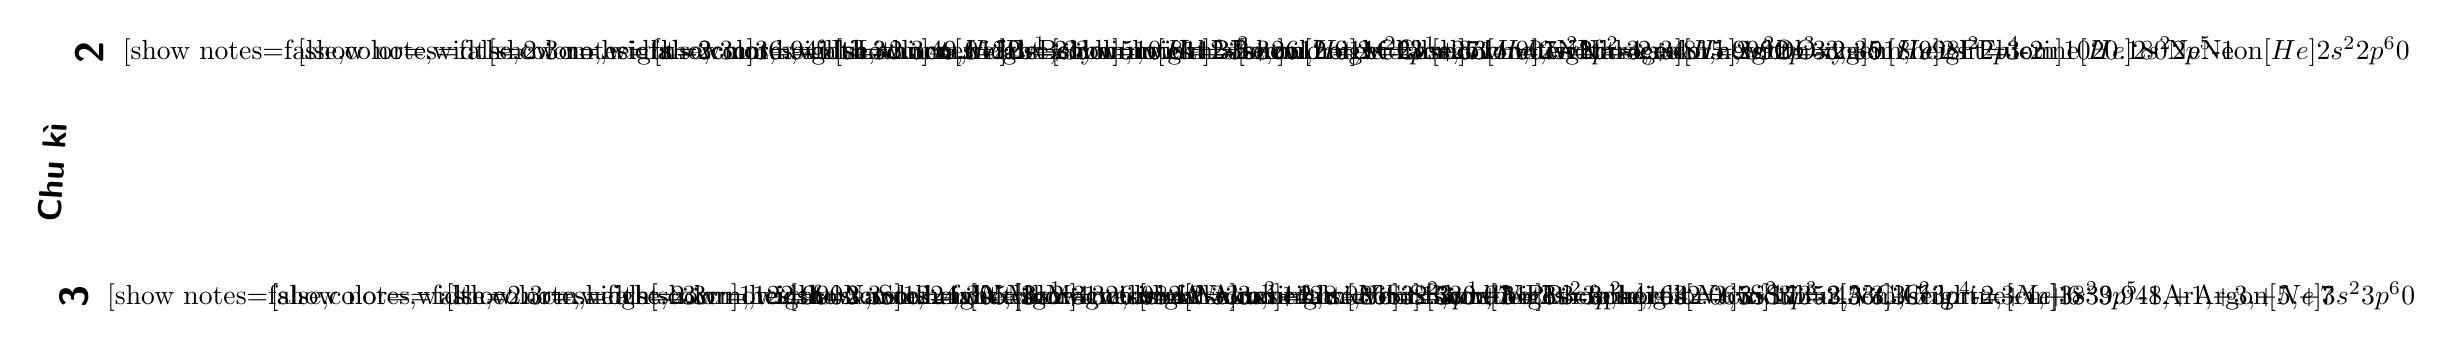
\begin{tikzpicture}[node distance=1mm]
		\foreach \num/\mass/\sym/\name/\config/\ox [count=\i from 1] in {
			3/6.941/Li/Lithium/$[He] 2s^1$/+1,
			4/9.012/Be/Beryllium/$[He] 2s^2$/+2,
			5/10.811/B/Boron/$[He]2s^2 2p^1$/+3,
			6/12.011/C/Carbon/$[He]2s^2 2p^2$/\text{-4,+4},
			7/14.007/N/Nitrogen/$[He]2s^2 2p^3$/\text{-3,+5},
			8/15.999/O/Oxygen/$[He]2s^2 2p^4$/-2,
			9/18.998/F/Fluorine/$[He]2s^2 2p^5$/-1,
			10/20.180/Ne/Neon/$[He]2s^2 2p^6$/0
		} {
			\path (\i*2.4cm,0) node[anchor=center] (element-2-\i) {
				\nguyento[show notes=false,color=\mauphu,width=2.3cm,height=3cm]{\num}{\mass}{\sym}{\name}{\config}{\ox}
			};
		}
		%%CK3
		\foreach \num/\mass/\sym/\name/\config/\ox [count=\i from 1] in {
			11/22.990/Na/Sodium/$[Ne] 3s^1$/+1,
			12/24.305/Mg/Magnesium/$[Ne] 3s^2$/+2,
			13/26.982/Al/Aluminium/$[Ne] 3s^2 3p^1$/+3,
			14/28.086/Si/Silicon/$[Ne] 3s^2 3p^2$/\text{-4,+4},
			15/30.974/P/Phosphorus/$[Ne] 3s^2 3p^3$/\text{-3,+3,+5},
			16/32.065/S/Sulfur/$[Ne] 3s^2 3p^4$/\text{-2,+4,+6},
			17/35.453/Cl/Chlorine/$[Ne]3s^23p^5$/\text{-1,+1,+3,+5,+7},
			18/39.948/Ar/Argon/$[Ne]3s^23p^6$/0
		} {
			\path (\i*2.4cm,-3.1cm) node[anchor=center] (element-3-\i) {
				\nguyento[show notes=false,color=\maunhan,width=2.3cm,height=3cm]{\num}{\mass}{\sym}{\name}{\config}{\ox}
			};
		}
		%%Thông tin chu kì
		\path (element-2-1.south west)--(element-2-1.north west) node[sloped,above,font=\Large\bfseries\sffamily,pos=0.5] (ck2){2};
		\path (element-3-1.south west)--(element-3-1.north west) node[sloped,above,font=\Large\bfseries\sffamily,pos=0.5] (ck3){3};
		\path (ck3)--(ck2) node[sloped,above=3pt,font=\large\bfseries\sffamily,pos=0.5] {Chu kì};
	\end{tikzpicture}
}
\captionof{figure}{Các nguyên tố thuộc chu kì 2 và chu kì 3 \label{fig:ck-2-3}}

\begin{hoivadap}
	\begin{cauhoi}
		Quan sát hình (\ref{fig:ck-2-3}) hãy cho biết số lớp electron các nguyên tố thuộc cùng chu kì
	\end{cauhoi}
\end{hoivadap}

\begin{ghinho}
	\indam{Chu kì} là tập hợp các nguyên tố có cùng số lớp electron.\\
	Bảng tuần hoàn có 7 chu kì:
	\begin{itemize}
		\item Chu kì 1,2,3 là chu kì nhỏ
		\item Chu kì 4,5,6,7 là chu kì lớn
	\end{itemize}
	\begin{center}
		\boxct{\indam{Số thứ tự chu kì = số lớp electron}}
	\end{center}
\end{ghinho}
\Noibat[\maunhan][][\faArrowCircleORight][]{Tìm hiểu về nhóm}
\begin{ghinho}
	\indam{Nhóm} là tập hợp các nguyên tố mà nguyên tử có cấu hình electron tương tự nhau (trừ nhóm VIIIB), do đó có tính chất hoá học gần giống nhau và được xếp theo cột.
	\begin{center}
		\boxct{\indam{Số thứ tự của nhóm A = số electron ở lớp ngoài cùng }}
	\end{center}
\end{ghinho}
\Noibat[\maunhan][][\faArrowCircleORight][]{Phân loại nguyên tố}
\begin{tomtat}
	Các nguyên tố hoá học cũng có thể được chia thành các khối như sau:
	\begin{itemize}
		\item  Khối các nguyên tố s gồm các nguyên tố thuộc nhóm IA và nhóm IIA, có cấu hình electron: [Khí hiếm] ns $\mathrm{s}^{1+2}$
		\item  Khối các nguyên tố p gồm các nguyên tố thuộc nhóm IIIA đến nhóm VIIIA (trừ nguyên tố He ), có cấu hình electron: [Khí hiếm] $\mathrm{ns}^2 \mathrm{np}^{1+6}$.
		\item  Khối các nguyên tố d gồm các nguyên tố thuộc nhóm B , có cấu hình electron: $\left[\right.$ Khí hiếm] $(\mathrm{n}-1) \mathrm{d}^{1+10} \mathrm{~ns}^{1+2}$.
		\item  Khối các nguyên tố f gồm các nguyên tố xếp thành hai hàng ở cuối bảng tuần hoàn, có cấu hình electron: [Khí hiếm] $(\mathrm{n}-2) \mathrm{f}^{0+14}(\mathrm{n}-1) \mathrm{d}^{0-2} \mathrm{~ns}$ (trong đó $\mathrm{n}=6$ và $\mathrm{n}=7$ ). Chúng gồm 14 nguyên tố họ Lanthanide (từ Ce đến Lu ) và 14 nguyên tố họ Actinide (từ Th đến Lr ).
	\end{itemize}
\end{tomtat}